\chapter{Introduction}
\label{chap:introduction}

% kind of problem statement in introduction
% positions required, but meshroom can be used
% scenes with highly specular objects trains better using log-transform
% discussion part: background color problem
% layer depth for NSVF can be way more shallow since voxel features
% assuming single(!) point(!) light only
% inverseCDF sampling for NSVF
% discrete regularization - noise to sigma field
% calculating normals from sigma and directly outputing normals


% light attenuation + light as learnable parameter (as there barely exist the ground truth value for real datasets)
% different sigma in voxel strategies for inVoxelApproximation


The task of reconstructing a real 3D scene from a set of 2D captured images
and modeling it under novel viewing and lighting conditions
is a long-standing problem in computer graphics and vision.
Possible complex scene geometries along with numerous appearance properties
make this task a tremendously challenging problem.
The real-world scenes contain a descent amount of complications
that can come from both the environment (e.g. illumination is not completely static)
and from the capturing hardware (e.g. distortions in camera lenses, low dynamic range (LDR) images).

The applications of realistic rendering include diverse fields,
such as visualization, animation, virtual and augmented reality, visual effects,
and even computer vision and robot navigation.

% \im{image here similar to in NeRF with the pipeline}

% Not very long about very basics
% \subsection{\{Rendering equation\} \im{or/and radiometry?}}
% \begin{enumerate}
%     %\item Color space \im{?}
%     \item LDR/HDR
%     \item Rendering equation
%     \item Transfer equation
%     \item (simple) volume rendering
%     \item BSSRDF + Reflection Models
% \end{enumerate}
% \sm{Not sure how relevant that is. Maybe put this in a subsection later for NeRF? Lowest priority for now.}

This task was traditionally addressed to the image-based rendering systems,
which use vision-based scene geometry together with the image-based view interpolation \cite{shumandkang2000}.
However, recent works in this field make use of deep neural networks
in order to learn implicit "neural" scene representation,
containing both geometric and appearance information. \cite{tewari2020state}

\cite{mildenhall2020nerf} presented a state-of-the-art approach,
which uses deep neural network as an implicit continuous volumetric scene representation.
In the core of this method lies the volume ray casting technique \cite{drebin1988volume},
which implies such volume processes as absorption and emission
while not accounting for scattering.
View rays are traced through the 2D captures of the scene,
sampled in a 3D space and then processed with neural network,
which predicts the volume density and color value at the given spatial point under a given viewing direction.
% These samples along the ray are used to estimate the rendering integral.
These samples along the ray are used to predict volume density and color value,
which are then gathered via alpha-compositing process.
This approach has quickly become a starting point for lots of other works \cite{liu2021neural, garbin2021fastnerf, reiser2021kilonerf, yu2021plenoctrees, rebain2020derf, lindell2021autoint}.
However, the main limitation for most of them is the lack of light interaction,
which disables the capabilities for rendering the scene under the novel light conditions.

\cite{bi2020neural} propose the NRF approach
that removes this limitation by reformulating the rendering equation in a way
that it accounts for the \textit{light transmittance},
i.e. the accumulated volume transmittance along corresponding light rays.
This approach only considers a single (but not static) point light source located on the scene.
However, the proposed implementation is only practical for one specific case
when the light source is co-located with the camera.
Although, this approach is already able to generalize for the relighting of the scene,
the predictions are still affected by a very sparse light-view space sampling
as there are only coincident light and view rays in the training dataset
(e.g. the model never deals with shadows on the training sample images).


% \section{Goal of the Thesis}
The goal of this thesis is to develop a solution
that is able to model scene geometry and appearance with view- and light-dependant effects
implying both co-located and non-colocated light sources.
This is done by utilizing the usage of neural sparse voxel fields (NSVF) \cite{liu2021neural}
with such a problem formulation that considers a single non-static point light source illumination \cite{bi2020neural}.
This method is called \textit{ExCol} (Explicit Colocated) and is only capable
to be processed within the co-located setting as in NRF approach.

In order to extend this setup for the non-colocated light setting, the \textit{ExBF} (Explicit Brute-Force) method is proposed,
which traces and samples light rays for each of the view sample points to calculate light transmittance values.
However, this approach is unrealistically slow and memory-demanding,
which makes it impractical.

It is proposed to solve this problem by an approximation scheme \textit{ExVA} (Explicit with in-Voxel Approximation),
which leverages the usage of voxel octree structure
and approximates light transmittance by the distance that light ray has travelled inside voxels.
This method seems to be able to perform at the same level of quality as the initial \textit{ExBF} scheme,
though drastically outperforming it in terms of efficiency.

Additionally the implicit neural reflectance representation \textit{ImNRF} is proposed,
which sacrifices controlling capabilities of the neural representation
for being the fastest implementation among presented schemes
and having less limitations in complexity of representing appearances.


To summarize, the contributions of this work are:
\begin{enumerate}
    \item An acceleration technique \textit{ExCol} for the NRF approach
    based on NSVF
    \item The approximation scheme \textit{ExVA}
    for the generalization \textit{ExBF} of proposed \textit{ExCol}
    that achieves comparable results with only a minor overhead
    \item The implicit scheme \textit{ImNRF} that extends NSVF to be able to learn light interaction
    \item Extension for these methods from LDR to HDR data
\end{enumerate}



% \section{Outline}
% In Chapter 2 related background along with already existing methods are described.

% Chapter 3 is dedicated to the proposed method.

% Chapter 4 describes and analyses the experiments and the results.


% \textit{Another difficulty is the low dynamic range (LDR) images
% that usually come as a result of capturing real-world scenes.
% LDR images can be under- or over-exposured, which definitely makes the problem harder.
% The high dynamic range (HDR) images can be achieved
% by capturing series of LR images with different exposure values
% and then blending them together into a single HDR image.
% However, this makes the whole process of retrieving real-world data highly complex. (\im{wanted to include this as 2nd paragraph, but too detailed, isnt it?})}




% This is the Introduction and this is a text citation to \textcite{bestpaper} where this is a citation in parentheses \parencite{bestpaper}.

% \begin{figure}[!ht]
%     \centering
%     \begin{subfigure}[t]{0.485\textwidth}
%         \centering
%         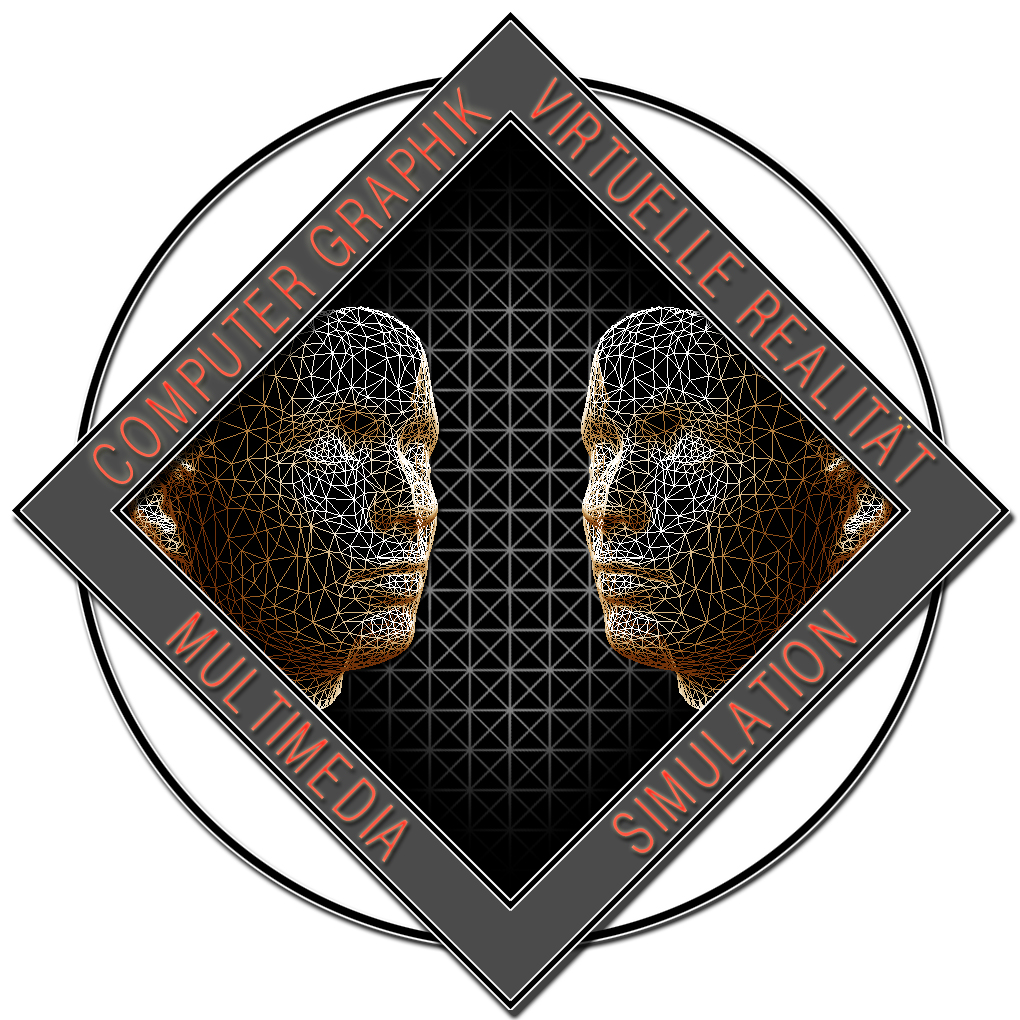
\includegraphics[height = 0.2\textheight, keepaspectratio]{logo_white.jpg}
%         \caption{The CG logo}
%         \label{fig:logo_sub_1}
%     \end{subfigure}
%     \begin{subfigure}[t]{0.485\textwidth}
%         \centering
%         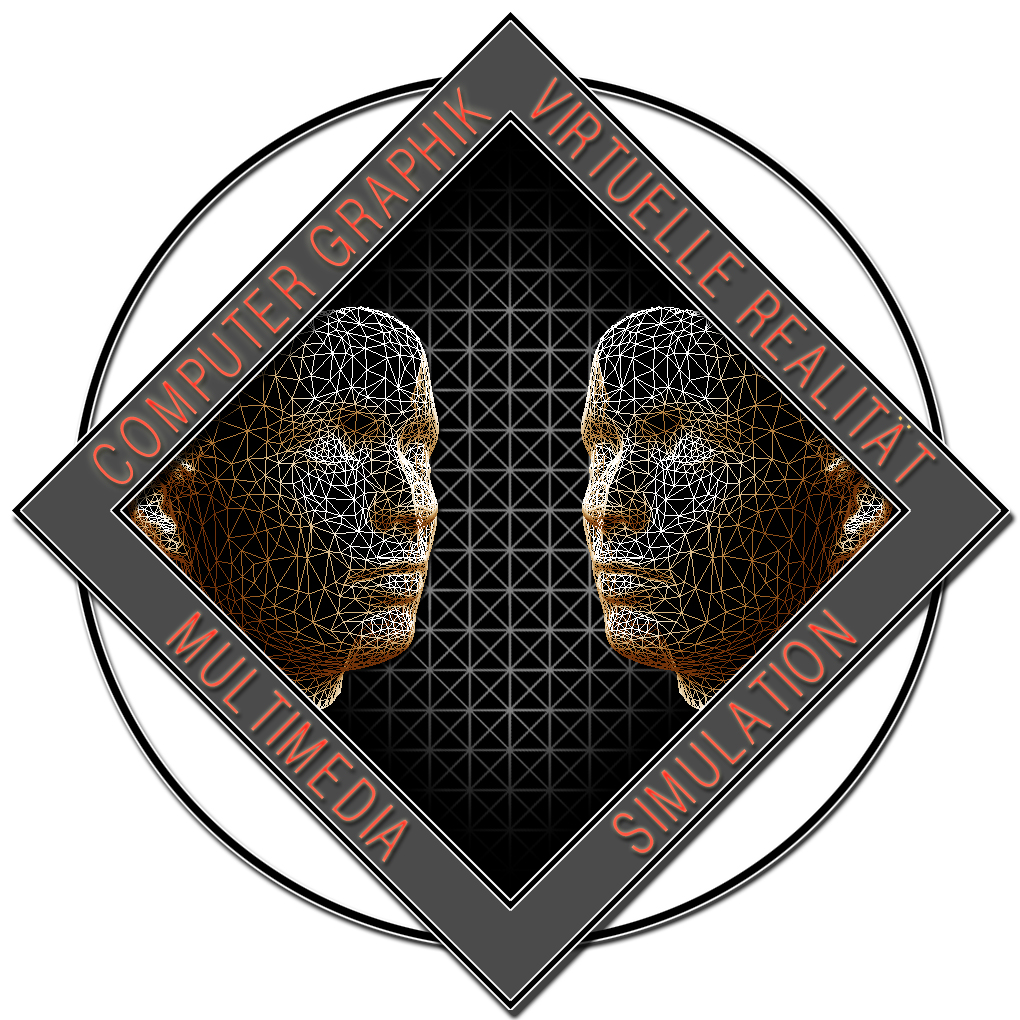
\includegraphics[height = 0.2\textheight, keepaspectratio]{logo_white.jpg}
%         \caption{The CG logo again}
%         \label{fig:logo_sub_2}
%     \end{subfigure}
%     \caption{The logo}
%     \label{fig:logo}
% \end{figure}

% So let us reference the logo above.

% cref : \cref{fig:logo} , \cref{fig:logo_sub_1} , \cref{fig:logo_sub_2}

% Cref : \Cref{fig:logo} , \Cref{fig:logo_sub_1} , \Cref{fig:logo_sub_2}


% \blankline
% Or reference the chapter.

% cref : \cref{chap:introduction}

% Cref : \Cref{chap:introduction}


% \lipsum[1]

% \begin{table*}[!htb]
%     \setArraystrech{1.5}
    
%     \centering
%     \caption{A fancy table showing some measured errors.}
%     \label{tab:benchmark}
%     \begin{tabular}{ L{0.2\textwidth}R{0.15\textwidth}R{0.15\textwidth}R{0.15\textwidth}R{0.15\textwidth}}
%     	\toprule
%     	Data sets                                    &   A &   B &   C &   D \\
%     	\addlinespace
%         \midrule
%         seq 1                                        & 0.1 & 0.2 & 0.3 & 0.4 \\
%     	seq 2                                        & 1.5 & 0.3 & 0.7 & 1.0 \\
%     	seq 3                                        & 0.4 & 0.7 & 9.4 & 0.9 \\ \bottomrule
%     \end{tabular}
% \end{table*}

% \lipsum[2]

